% 1977 年云南卷参考题 1：有盖圆柱形氨水池示意图，虚线轴上标高 h，
% 顶面自圆心画一段半径（按源卷第 4 页布局）
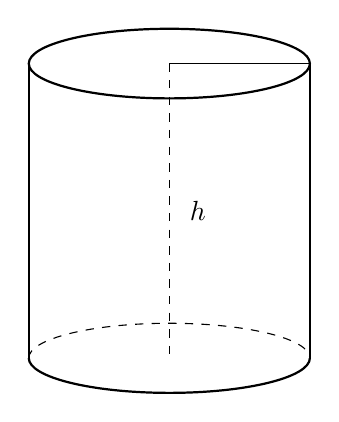
\begin{tikzpicture}[scale=1.7]
  \draw[thick] (0,2.2) ellipse (1.05 and 0.26);
  \draw[thick] (-1.05,0)--(-1.05,2.2);
  \draw[thick] (1.05,0)--(1.05,2.2);
  \draw[thick] (-1.05,0) arc (180:360:1.05 and 0.26);
  \draw[dashed] (-1.05,0) arc (180:0:1.05 and 0.26);
  \draw[thin] (0,2.2)--(1.05,2.2);
  \draw[dashed] (0,2.2)--(0,0);
  \node[right] at (0.08,1.1) {$h$};
\end{tikzpicture}
